\section{Usage Example}

% ANTOINE -> TODO

% TODO - from reviewer 2 : Case study should be about real systems, not a toy example which suddenly enforces all the maturity restrictions (why such a naive system would be so constrained (maturity D3-S2-P2)?). You could provide insights about a case in your company XXX. Or ask for developer's feedback with real-world systems.

% TODO - from reviewer 2 : Individual figures (Users, Playlists, Songs) take too much space, they can be replaced for a single Table or Figure (Class diagram-esque).

% TODO - from reviewer 2 : How did you define the criteria (a.k.a. the list of unknown acronyms) that the technology for your case study should meet(beginning of Sec. 5.2, 5.3 and 5.4)? those seem to be pulled out from thin air.

This section illustrates the usage of the presented classification matrix to build a system with a targeted maturity level in mind.

\subsection{Example system presentation}

The system we use for this example almost targets the highest maturity of WS3 (D3-S2-P2). Indeed, it does not target to meet the Atomic Resources constraint. It is a music sharing API that allows one to search for songs and playlists. Logged in users can submit songs that will be reviewed by administrators of the platform. If accepted, songs will become publicly available. Songs and playlists have three states: (i) submitted, (ii) accepted or (iii) rejected. Besides that, each user can create up to ten playlists.

Therefore, this API has six types of resources: (i) user, (ii) collection of users, (iii) song, (iv) collection of songs, (v) playlist and (vi) collection of playlists. These types are presented as a resource model in figures 1--3.

Each collection of another type of resource contains a \textit{listAll...(filters)} operation. For the purpose of this paper, we consider that \textit{filters} corresponds to the query parameters of the URI. For example \textit{myapi.com/songs?title=foo\&artist=bar} results in \textit{filters} having a field \textit{title} with value \textit{foo} and another one \textit{artist} with value \textit{bar}. We consider that a collection can be filtered on each property of the resource type it holds. So, \textit{Songs} have \textit{id}, \textit{artist}, \textit{title} and \textit{file} filters.

\begin{figure}[ht]
\caption{Users resource model}
\centering
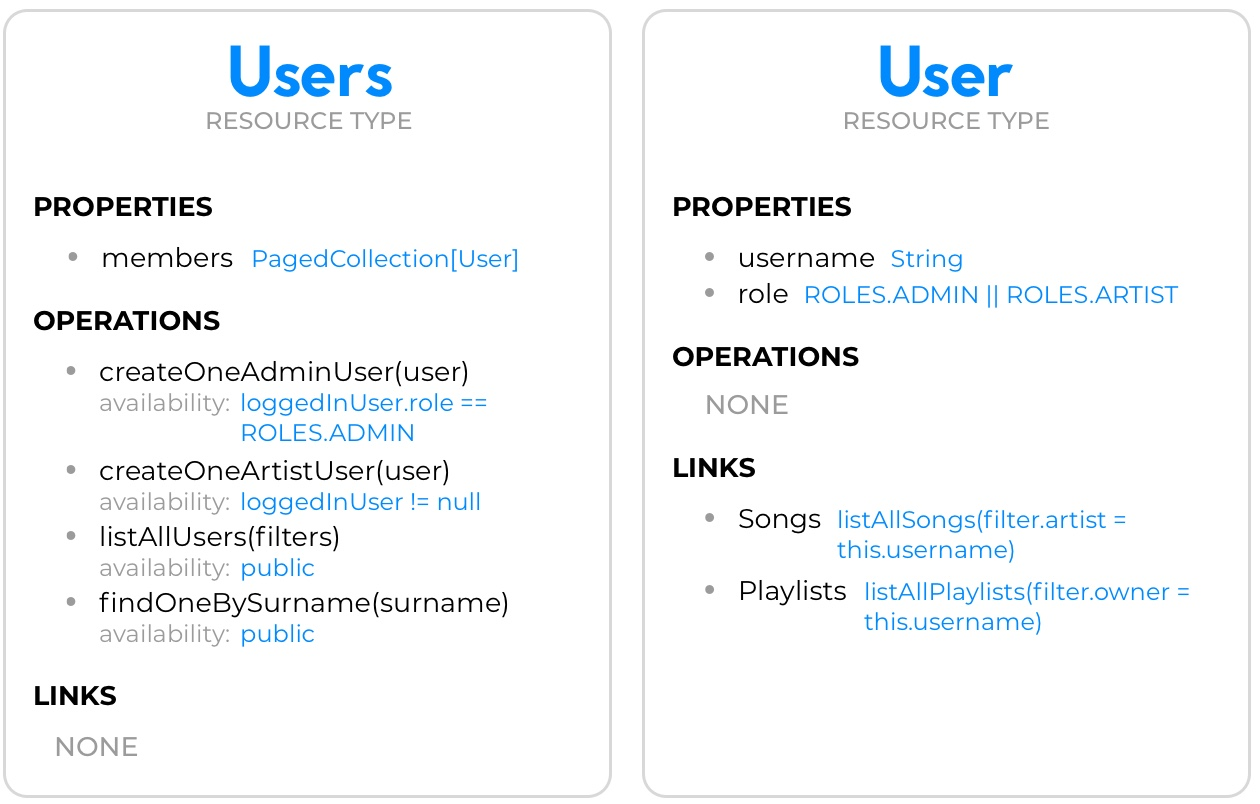
\includegraphics[width=0.47\textwidth]{figures/users.jpg}
\end{figure}

\begin{figure}[ht]
\caption{Playlists resource model}
\centering
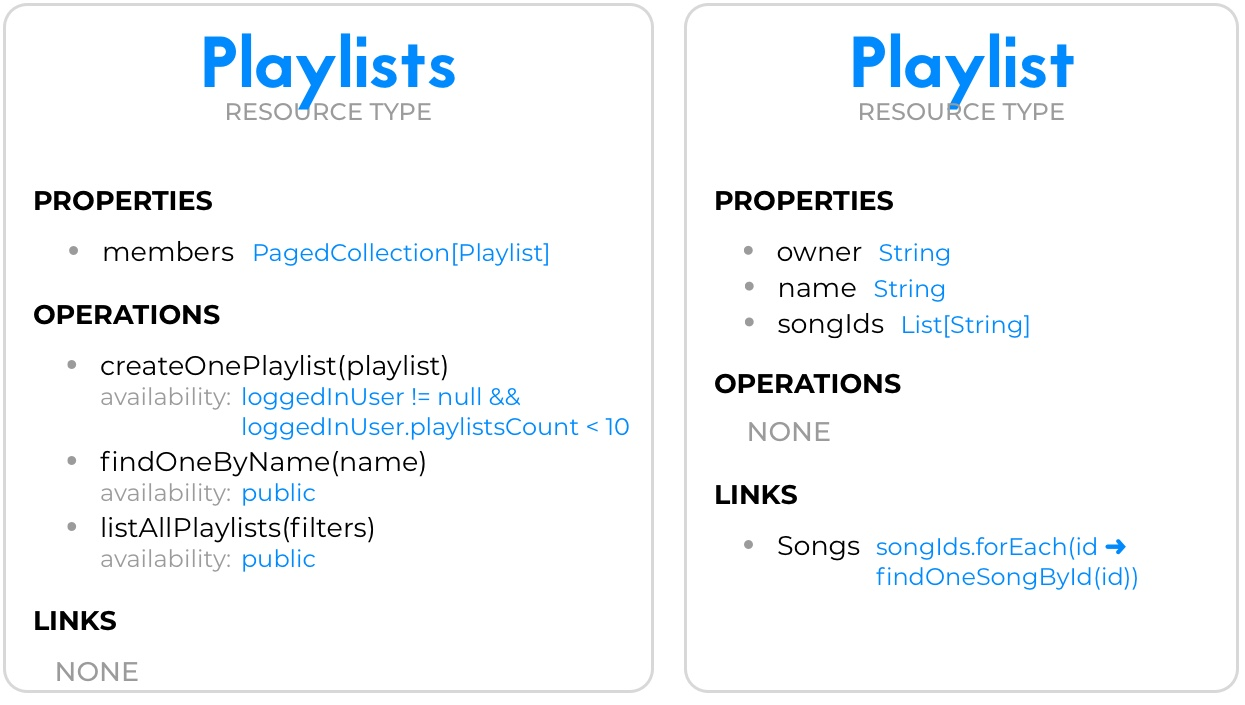
\includegraphics[width=0.44\textwidth]{figures/playlists.jpg}
\end{figure}

\begin{figure}[ht]
\caption{Songs resource model}
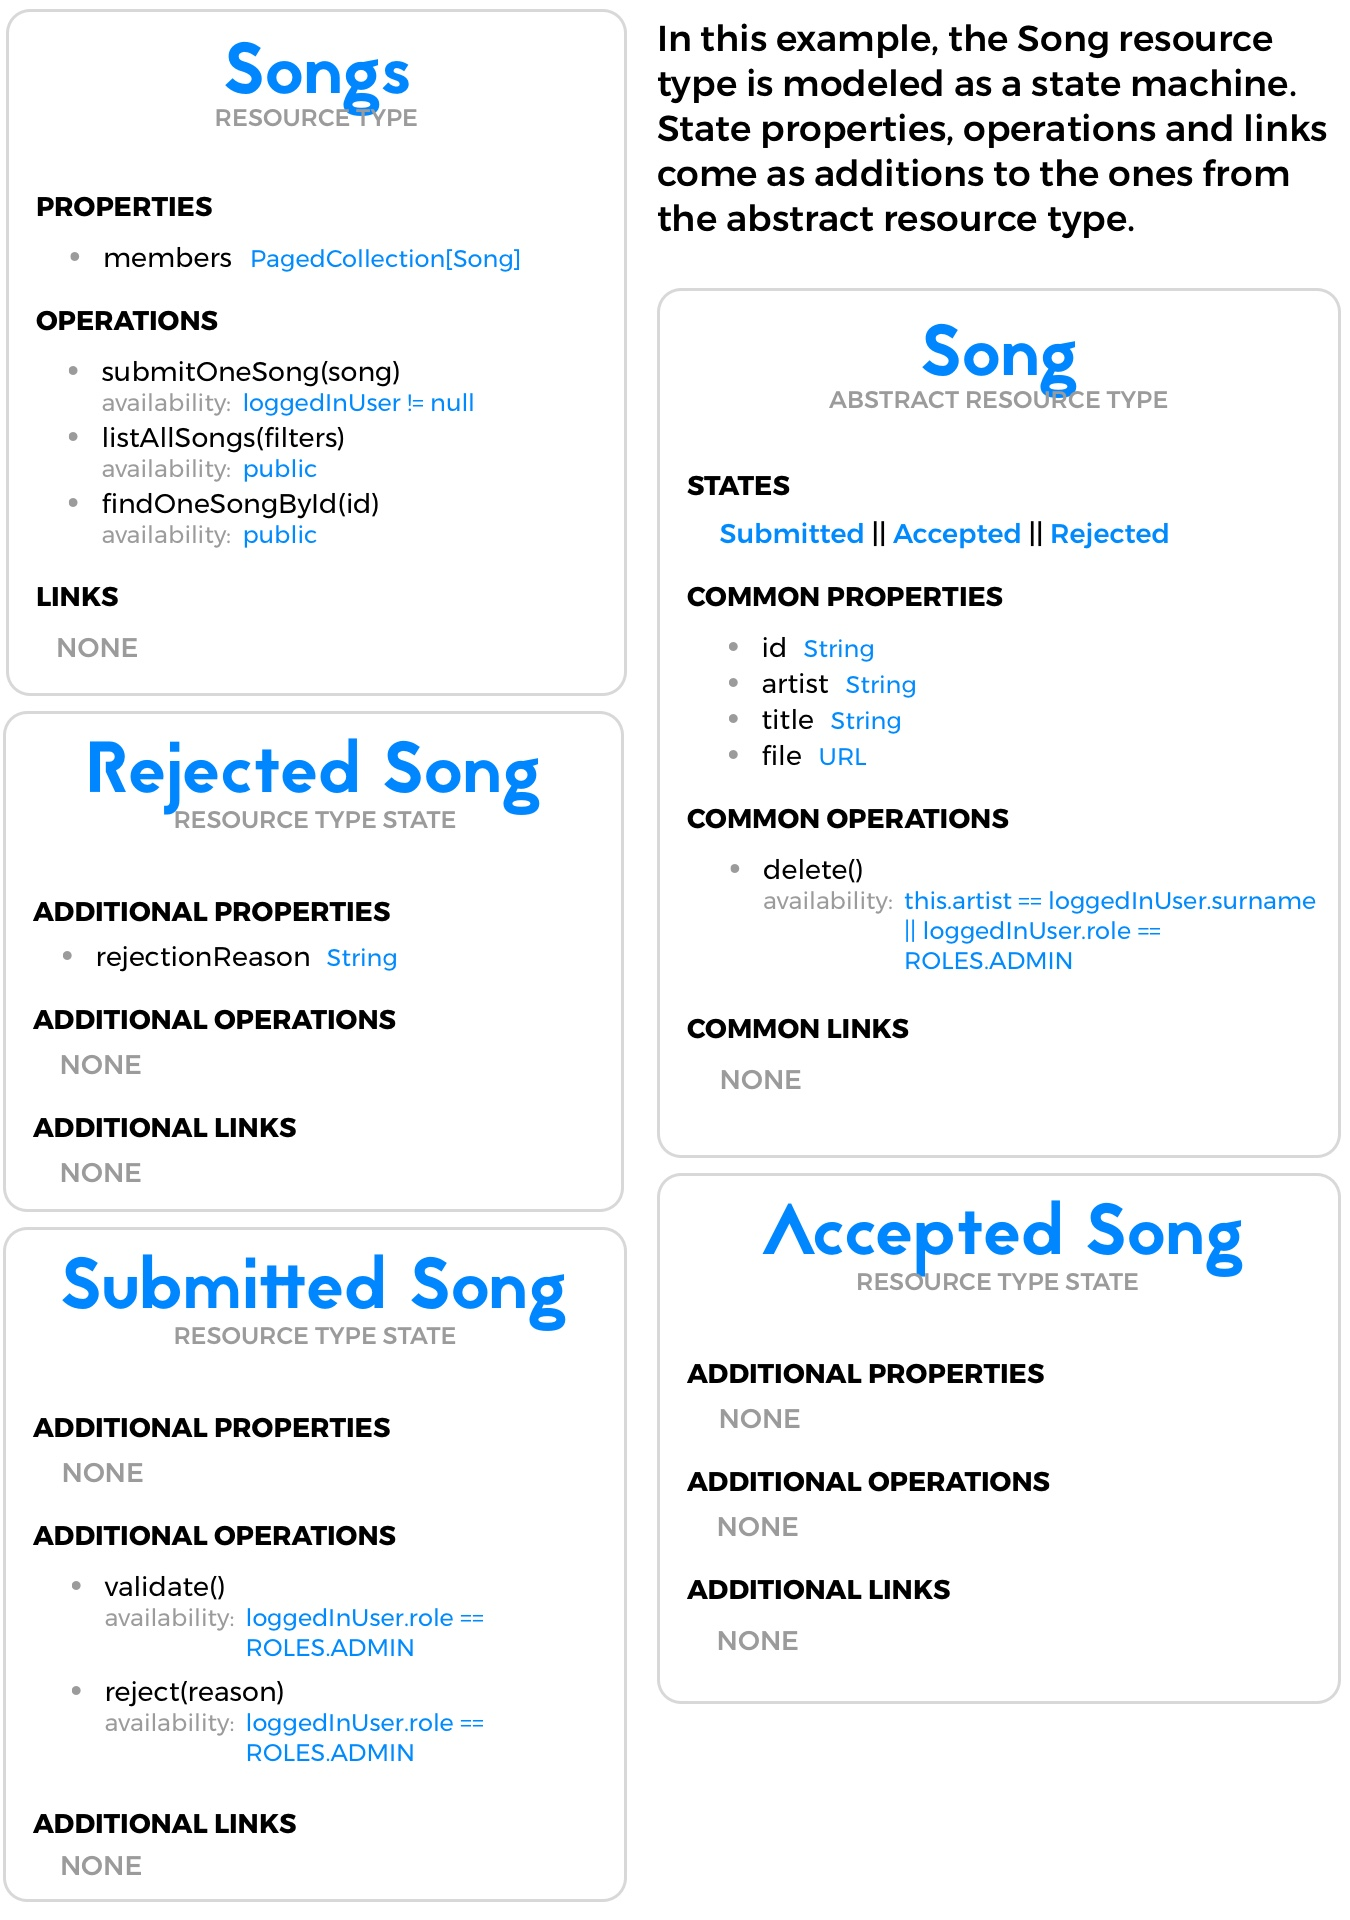
\includegraphics[width=0.44\textwidth]{figures/songs.jpg}
\end{figure}

The domain of this API has four more constraints that are not represented on the resource model. They are:

\begin{itemize}
    \item Calling \textit{Songs.submitOne(song)} as an admin will create an AcceptedSong;
    \item Calling \textit{Songs.submitOne(song)} as an artist will create a SubmittedSong;
    \item A \textit{Playlist.name} can be composed only of characters, spaces and numbers;
    \item A \textit{User.surname} can be composed only of characters, dots and numbers.
\end{itemize}

On the \textit{Profile} aspects, the system should (i) advertise the resource's state explicitly, (ii) provide a documentation of resources and operations, (iii) document its authentication mechanism, (iv) document all information visible in the resource model and (v) support HATEOAS. Each documentation must be machine-processable.

On the \textit{Semantic} aspects, the system should (i) propose an RDF format, to be compatible with the Semantic Web, (ii) link data to others using RDF vocabulary to express relationships and (iii) provide the semantic of the data, their properties and operations.

This system targets humans first, while still requiring machine-interpretability, and must send hypermedia controls through a JSON format. Offering only one interchange format is sufficient.

\subsection{Finding the appropriate Interface Description Language}

To find the most appropriate Interface Description Language to this system, we first need to find the criteria that the technologies we are looking for should meet. In this scenario, they are: \textit{MR, MRA, MRO, OTO, DR, OSD, LT, HL, HYP, MC, COA, CC, AUT, SD, DC, RDF, CL} and \textit{SCL}. The plus are: \textit{SC, RUN, PS} and \textit{RS}. It is a total of 22 criteria.

% TODO - From reviewer 1 : in Section 5.2, the example needs to consider 22 criteria, but there is no justification why the criteria should be considered when implementing the example

The three technologies that meet the highest number of these criteria are: Hydra (15), the model presented in Modeling RESTful Applications \cite{Schreier:2011:MRA:1967428.1967434} (12) and WSDL+SAWSDL (10). In this scenario, the architect would have to make his decision depending on how important and costly to implement are the features that are not supported by the technologies.

% TODO - From reviewer 1 : it is not clear why the three technologies are good because these technologies do not satisfy some criteria

\subsection{Finding the appropriate data-interchange format}

For this category, the criteria technologies should meet are: \textit{LT, CM, OSD, DR, PS, CL, SCL, RDF, JSON, HL, HYP} and \textit{RC}. The plus are: \textit{NOM, HF, PX, ECD} and \textit{CUR}. It is a total of 17 criteria. In addition to meet as much criteria as possible, the interchange format should be compatible with the IDL chosen at the previous step. This is particularly important when an RDF IDL has been chosen as it lowers the number of functionality provided by each technology, making them easier to replace.

The three technologies that meet these criteria best are: Mason, JSON-LD with Hydra, and Siren. JSON-LD is the only one JSON  format designed for RDF, even though others support adding vocabulary. Combined with Hydra they meet 15/17 criteria. Mason meet 15 criteria and Siren 10. This time, selection depends on the chosen IDL, or might influence the IDL choice.

Mason and JSON-LD with Hydra meet the highest number of criteria. Because JSON-LD is the only one RDF format in the list, it makes it a more interesting option. However, each technology leaves non-supported features that the development team will have to implement by itself.

\subsection{Finding the appropriate development framework}

In this scenario, an architect would be looking for a framework that meet the criteria \textit{SC, OTO, MRO, EXT, DR, OSD, LT, PS, HL, HYP, MC, LNM, COA, CC, AUT, ERR, SD, DC, RDF, CL} and \textit{SCL}. If a framework already supports the previously chosen IDL and data-interchange format, it would be a plus and \textit{EXT} would become unnecessary.

From those criteria, the technology that meet the highest number of criteria is API Platform with 18, A framework for semantic description of RESTful APIs comes second with 14 and Spring HATEOAS with 10. In this scenario, an architect would likely opt for API Platform.

\subsection{Results}

% TODO - from reviewer 2 : Section says that "the choice is not straightforward because no technology meet al the criteria" but in the next sentence you just select one for each category! how do you support such decision? which are the particular "context of the project" circumstances that led you to do so? That's why I'd prefer a real case study with real constraints. 

% TODO - from reviewer 2 : Apart from that, a "results" section with only one paragraph and no actual finding does not give that much for the reader and could be removed.

In this section we gave an example showing how to use the proposed classification matrix. Even though the choice is not straightforward because no technology meet all the criteria, it is easy to reduce the number of candidate to three, and then make an informed decision based on the context of the project.
From this scenario, we would have gone with Hydra, JSON-LD and API-platform.
